\loesung{
\begin{table}[H]
		\centering
		\begin{tabular}{clr}
			\hline
			iteration & baselearner & risk\_reduction \\ 
			\hline
			1 & days\_since\_2011 & 140 782.94 \\ 
			2 & temp & 135 986.35 \\ 
			3 & days\_since\_2011 & 110 314.74 \\ 
			4 & temp & 106 854.21 \\ 
			5 & temp & 86 551.91 \\ 
			\hline
		\end{tabular}
	\end{table}	
	In the above table, the difference in risk (i.e. the risk reduction) in each iteration is given. 
	The importance of a given feature can be calculated by summing up these differences over all iterations corresponding to this feature (equivalent to the different base learners in this case, since each base learner only uses one feature).
    The final feature importances look like this: 
	
	\begin{minipage}[t]{0.45\textwidth}
		\vspace{-2.5cm}
			\begin{tabular}{lr}
				\hline
				feature & risk\_reduction \\ 
				\hline
				days\_since\_2011 & 251 097.68 \\ 
				temp & 329 392.47 \\ 
				\hline
			\end{tabular}

	\end{minipage}
	\begin{minipage}[t]{0.45\textwidth}
		
		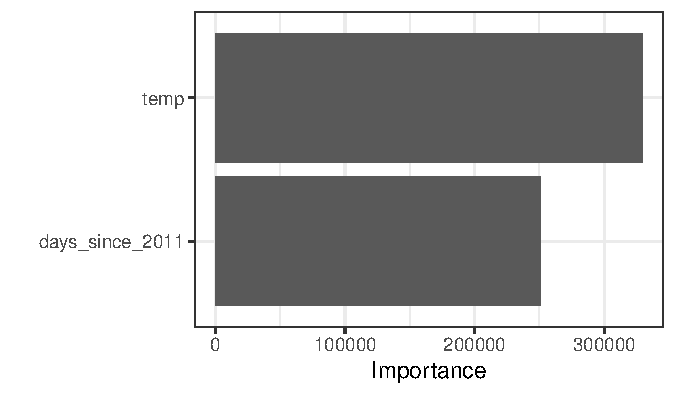
\includegraphics[width = .8\textwidth]{figure/compboost_pfi.pdf}
		
	\end{minipage}


}
